\documentclass[12pt,english,]{article}
\usepackage{lmodern}
\usepackage{amssymb,amsmath}
\usepackage{ifxetex,ifluatex}
\usepackage{fixltx2e} % provides \textsubscript
\ifnum 0\ifxetex 1\fi\ifluatex 1\fi=0 % if pdftex
  \usepackage[T1]{fontenc}
  \usepackage[utf8]{inputenc}
  \usepackage{textcomp} % provides euro and other symbols
\else % if luatex or xelatex
  \usepackage{unicode-math}
  \defaultfontfeatures{Ligatures=TeX,Scale=MatchLowercase}
\fi
% use upquote if available, for straight quotes in verbatim environments
\IfFileExists{upquote.sty}{\usepackage{upquote}}{}
% use microtype if available
\IfFileExists{microtype.sty}{%
\usepackage[]{microtype}
\UseMicrotypeSet[protrusion]{basicmath} % disable protrusion for tt fonts
}{}
\usepackage{hyperref}
\hypersetup{
            pdfauthor={Thinh Truong},
            pdfborder={0 0 0},
            breaklinks=true}
\urlstyle{same}  % don't use monospace font for urls
\usepackage[margin=1in]{geometry}
\usepackage{graphicx,grffile}
\makeatletter
\def\maxwidth{\ifdim\Gin@nat@width>\linewidth\linewidth\else\Gin@nat@width\fi}
\def\maxheight{\ifdim\Gin@nat@height>\textheight\textheight\else\Gin@nat@height\fi}
\makeatother
% Scale images if necessary, so that they will not overflow the page
% margins by default, and it is still possible to overwrite the defaults
% using explicit options in \includegraphics[width, height, ...]{}
\setkeys{Gin}{width=\maxwidth,height=\maxheight,keepaspectratio}
\setlength{\emergencystretch}{3em}  % prevent overfull lines
\providecommand{\tightlist}{%
  \setlength{\itemsep}{0pt}\setlength{\parskip}{0pt}}
\setcounter{secnumdepth}{0}
% Redefines (sub)paragraphs to behave more like sections
\ifx\paragraph\undefined\else
\let\oldparagraph\paragraph
\renewcommand{\paragraph}[1]{\oldparagraph{#1}\mbox{}}
\fi
\ifx\subparagraph\undefined\else
\let\oldsubparagraph\subparagraph
\renewcommand{\subparagraph}[1]{\oldsubparagraph{#1}\mbox{}}
\fi

% set default figure placement to htbp
\makeatletter
\def\fps@figure{htbp}
\makeatother

\usepackage{float}
\usepackage[boxruled,vlined]{algorithm2e}
\usepackage{listings}
\usepackage{xcolor}
\usepackage {tikz}
\usepackage{indentfirst}
\usepackage{tabularx}
\usepackage{multirow}
\usepackage{pgfplots}
%\usepackage[bottom]{footmisc}
\colorlet{mygray}{black!30}
\colorlet{mygreen}{green!60!black}
\colorlet{mymauve}{red!90}

\lstset{
  tabsize=2,
  backgroundcolor=\color{gray!10},  
  basicstyle=\ttfamily,
  columns=fullflexible,
  breakatwhitespace=false,      
  breaklines=true,                
  captionpos=b,                    
  commentstyle=\color{mygreen}, 
  extendedchars=true,              
  frame=single,                   
  keepspaces=true,
  morekeywords={self},
  keywordstyle=\bfseries\color{blue},      
  language=python,                 
  numbers=left,                
  numbersep=5pt,
  breaklines=true,
  numberstyle=\tiny, 
  rulecolor=\color{mygray},        
  showspaces=false,               
  showtabs=true,
  emph={__init__},
  emphstyle=\color{mymauve},
  stringstyle=\color{mymauve},                          
  title=\lstname                
}

\definecolor{light-gray}{gray}{0.9}
\newcommand{\code}[1]{\colorbox{light-gray}{\texttt{#1}}}
\newcommand{\pnt}[1]{{\scriptstyle#1}}
\let\origfigure\figure
\let\endorigfigure\endfigure
\renewenvironment{figure}[1][2] {
    \expandafter\origfigure\expandafter[H]
} {
    \endorigfigure
}
\usepackage{etoolbox}
\makeatletter
\providecommand{\subtitle}[1]{% add subtitle to \maketitle
  \apptocmd{\@title}{\par {\large #1 \par}}{}{}
}
\makeatother
\ifnum 0\ifxetex 1\fi\ifluatex 1\fi=0 % if pdftex
  \usepackage[shorthands=off,main=english]{babel}
\else
  % load polyglossia as late as possible as it *could* call bidi if RTL lang (e.g. Hebrew or Arabic)
  \usepackage{polyglossia}
  \setmainlanguage[]{english}
\fi

\title{\textbf{Project Report}\\
\Large{An Implementation Of:}}
\providecommand{\subtitle}[1]{}
\subtitle{Fractional Cascading Algorithm on N-ary Trees}
\author{Thinh Truong}
\date{13 December 2023}

\begin{document}
\maketitle

\hypertarget{section1}{%
\section{\texorpdfstring{1
\enspace Introduction}{1 Introduction}}\label{section1}}

Implementation of an algorithm helps us observe its efficiency and behavior in practice.
With the goal to improve running time of naive algorithm on a N-ary tree problem, we explore 
fractional cascading algorithm. \\

Consider an undirected connected graph $G= (V,E)$ with k vertices. Let $d$ be the maximal
degree of any vertex, assumed to be a constant. Each vertex $v$ contains a sorted list $C(v)$
of real numbers. The type of query we want to solve is: Given a real number $y$ and a
connected subgraph $(V', E')$ of G, locate $y$ in all lists $C(v)$ for $v \in V'$. \\

Let $n$ be the sum of the lengths of all lists $C(v)$. By performing a binary search in
$C(v)$ for each $v \in V'$, we can solve the query in $O(|V'|\log_{} n)$ time, and the amount
of space used is $O(n+k)$.\\ 

Fractional cascading can improve this running time to $O(|V'|+\log_{} n)$ while still using 
$O(n+k)$ space. The technique was initially introduced by Chazelle and Guibas, but the 
original version is deterministic and quite complicated. Hence, this report will focus on an
easier approach of the algorithm which is the randomized fractional cascading technique, due 
to Kurt Mehlhorn in 1991. In this report, I will briefly explain each part of the randomized 
fractional cascading technique on N-ary tree, show the implementation along with the 
practical running time analysis. \\

\newpage


\hypertarget{section2}{%
\section{\texorpdfstring{2 \enspace The Implementation}{2 The Implementation}}\label{section2}}

The implementation of the algorithm and its components will be described and explained 
throughout this section.

\hypertarget{section2.1}{%
\subsection{\texorpdfstring{2.1 Node classes and functions}{2.1 Node classes and functions}}\label{section2.1}}

I use the \code{TreeNode} class to represent each node in the tree.

~

\begin{lstlisting}
class TreeNode:
    def __init__(self, value, max_list_len: int):
        self.value = value
        self.parent : TreeNode = None
        self.children : list[TreeNode] = []
        self.node_list = sorted([random.randint(MIN_NUMBER_IN_LIST, MAX_NUMBER_IN_LIST) for _ in range(random.randint(1, random.randint(1, max_list_len)))])
        self.augmented_list= [ListNode(MIN_BOUNDARY, self)] + [ListNode(MAX_BOUNDARY, self)]     #initialize the list with boundary values

        # set prev/next pointers for augmented_list
        for i in range(len(self.augmented_list)):
            if i > 0:
                self.augmented_list[i].set_prev(self.augmented_list[i-1])
            if i < len(self.augmented_list) - 1:
                self.augmented_list[i].set_next(self.augmented_list[i+1])

    def add_child(self, child_node: "TreeNode"):
        self.children.append(child_node)

    # generate augmented list without having proper pointer set
    def generate_augmented_list(self):
        # connect boundaries by bridges to neighbors
        for child in self.children:
            self.augmented_list[0].add_bridges(child.augmented_list[0])
            child.augmented_list[0].add_bridges(self.augmented_list[0])
            self.augmented_list[-1].add_bridges(child.augmented_list[-1])
            child.augmented_list[-1].add_bridges(self.augmented_list[-1])
        if self.parent:
            self.augmented_list[0].add_bridges(self.parent.augmented_list[0])        
            self.parent.augmented_list[0].add_bridges(self.augmented_list[0])   
            self.augmented_list[-1].add_bridges(self.parent.augmented_list[-1])
            self.parent.augmented_list[-1].add_bridges(self.augmented_list[-1])
        # perform insert on neighbors
        for value in self.node_list:
            list_node = insert_own_list(self.augmented_list, value, self)
            if list_node != None:
                insert_recursive(list_node, self)

    def post_processing(self):
        # set proper pointers
        start, end = 0, 0
        for i in range(len(self.augmented_list)):
            if self.augmented_list[i].tree_node:
                end = i
                current_proper = self.augmented_list[i]

                while start <= end:
                    self.augmented_list[start].set_proper(i, current_proper)
                    start += 1

        # add boundary values on node_list for naive algorithm
        self.node_list.insert(0, MIN_BOUNDARY)
        self.node_list.append(MAX_BOUNDARY)

    def print_augmented_list(self):
        values = list(map(lambda node: node.value, self.augmented_list))
        return values

\end{lstlisting}
\vspace{-9truemm}
\begin{minipage}{1\textwidth}
  \begin{flushright}
  {\footnotesize \emph{Source \footnotemark: fractional-cascading/src/node.py }\par}
  \end{flushright}
\end{minipage}
\vspace{0.5truemm}
\footnotetext{Path to the source file in the implementation's GitHub repository.}

Each \code{TreeNode} $v$ contains \code{parent} and \code{child} attributes. It also
stores  \code{node\_list} which represents a sorted list $C(v)$ of real numbers, and 
\code{augmented\_list} which represents the augmented list $A(v)$. The 
\code{generate\_augmented\_list()} function can be called to generate $A(v)$ list from $C(v)$ 
list, and \code{post\_processing()} can be used to set the proper pointers and after $A(v)$ 
list is generated. \\

Each element in $A(v)$ list is represented by a \code{ListNode}.

~

\begin{lstlisting}
class ListNode:
    def __init__(self, value, tree_node: TreeNode = None):
        self.value = value
        self.tree_node = tree_node
        self.bridges : list["ListNode"] = []
        self.prev = None
        self.next = None
        self.proper = None
    
    def add_bridges(self, list_node: "ListNode"):
        self.bridges.append(list_node)

    def set_prev(self, list_node: "ListNode"):
        self.prev = list_node

    def set_next(self, list_node: "ListNode"):
        self.next = list_node
    
    # Save proper as (index, list_node)
    def set_proper(self, index: int, list_node: "ListNode"):
        self.proper = (index, list_node)
\end{lstlisting}
\vspace{-9truemm}
\begin{minipage}{1\textwidth}
  \begin{flushright}
  {\footnotesize \emph{Source: fractional-cascading/src/node.py }\par}
  \end{flushright}
\end{minipage}
\vspace{0.5truemm}

Each element \code{ListNode} in $A(v)$ stores the pred, next, proper and bridge pointers. Using \code{TreeNode} and \code{ListNode}, with the help of helper functions, we can create a balanced N-ary tree with \code{create\_whole\_tree()} which takes the size of the tree and maximum degree of a node as parameters.

\hypertarget{section2.2}{%
\subsection{\texorpdfstring{2.2 Path functions}{2.2 Path functions}}\label{section2.2}}

We want to the the algorithm using two different paths. The first one is a random path from 
the root to a leaf. The second one is a random path from a leaf going up to a random node in 
the middle of the tree, and then going down to a random leaf. Throughout the paper, the root 
to leaf path will be referred as path 1, and the other path will be referred as path 2. These
paths are generated by the following functions.

~

\begin{lstlisting}
def root_to_leaf_path(root: TreeNode, node_degree: int):
    if not root:
        return []
    
    path = []
    current = root

    while current:
        path.append(current)

        if not current.children:
            break

        child_index = random.randint(0, node_degree - 2)
        current = current.children[child_index]

    return path

def get_leaf_nodes(root: TreeNode):
    leaf_nodes: list[TreeNode] = []

    def dfs(node: TreeNode):
        if not node:
            return
        if not node.children:
            leaf_nodes.append(node)
        for child in node.children:
            dfs(child)

    dfs(root)
    return leaf_nodes

def leaf_node_leaf_path(root: TreeNode, height: int):
    leaf_nodes = get_leaf_nodes(root)

    if not leaf_nodes:
        return []
    
    # Select a random starting leaf node
    start_leaf = random.choice(leaf_nodes)

    path = []
    current = start_leaf
    path.append(current)

    mid_point = height//2

    # Path going up
    for _ in range(mid_point):
        if current.parent:
            current = current.parent
            path.append(current)

    # Path going down
    for _ in range(mid_point):
        if current.children:
            current = random.choice(current.children)
            path.append(current)

    return path
\end{lstlisting}
\vspace{-9truemm}
\begin{minipage}{1\textwidth}
  \begin{flushright}
  {\footnotesize \emph{Source: fractional-cascading/src/paths.py }\par}
  \end{flushright}
\end{minipage}
\vspace{0.5truemm}

Given a N-ary tree of size $n$ where $n$ is even, path 1 will produce a path of $n/2$ nodes 
while path 2 will produce a path of $(n/2) +1$ nodes. For example, with $n=4$, the path 
produced by path 1 has length of 4 while the path produced by path 2 has length of 5. When 
$n$ is odd, the length of the paths produced by the two techniques will be the same.

\hypertarget{section2.3}{%
\subsection{\texorpdfstring{2.3 Algorithm functions}{2.3 Algorithm functions}}\label{section2.3}}

~

\begin{lstlisting}
def naive_algorithm(path: list[TreeNode], target: int):
    result = []
    for tree_node in path:
        # binary seach
        search_result = binary_search_naive(tree_node.node_list, target)
        result.append(search_result)
    return result

def binary_search_naive(lst, target):
    left, right = 0, len(lst) - 1

    while left < right:
        mid = (left + right) // 2

        if lst[mid] == target:
            return target
        elif lst[mid] < target:
            left = mid + 1
        else:
            right = mid

    return lst[right] 
\end{lstlisting}
\vspace{-9truemm}
\begin{minipage}{1\textwidth}
  \begin{flushright}
  {\footnotesize \emph{Source: fractional-cascading/src/algorithms.py }\par}
  \end{flushright}
\end{minipage}
\vspace{0.5truemm}

~

\begin{lstlisting}
def fractional_cascading(path: list[TreeNode], target: int):
    result = []

    # Binary search on first tree node
    current_node = path[0]
    (first_index, first_value) = binary_search_fc(current_node.augmented_list, target)
    if first_value == target and current_node.augmented_list[first_index].tree_node:
        result.append(first_value)
    else:
        result.append(current_node.augmented_list[first_index].proper[1].value)

    cur_index = first_index
    # fractional cascading on other nodes
    for i in range(len(path)-1):
        cur_index, res = helper(cur_index, path[i], path[i+1], target)
        result.append(res)

    return result

def binary_search_fc(lst: list[ListNode], target: int):
    #return (index, value)
    left, right = 0, len(lst) - 1

    while left < right:
        mid = (left + right) // 2

        if lst[mid].value == target:
            return (mid, target)
        elif lst[mid].value < target:
            left = mid + 1
        else:
            right = mid 
    return (right, lst[right].value)

def helper(cur_index: int, cur_node: TreeNode, next_node: TreeNode, target: int):
    cur_list = cur_node.augmented_list
    current = cur_list[cur_index]
    found = False
    value = 0
    while current:
        if current.bridges:
            for bridge in current.bridges:
                if bridge.tree_node == next_node: #step 2
                    current = bridge #step 3
                    found = True
                    break
        if found:
            break
        else:
            current = current.next
    value = current.proper[1].value
    while current and current.prev.value >= target: #step 4
        current = current.prev
        if current.proper:
            value = current.proper[1].value
    
    index = next_node.augmented_list.index(current)

    if current.proper and value == target:
        return (index, target) # return index of current element in A(v), and matching value in C(v)

    return (index, value) # return index of element in A(v), and smallest value in C(v) that is greater target
\end{lstlisting}
\vspace{-9truemm}
\begin{minipage}{1\textwidth}
  \begin{flushright}
  {\footnotesize \emph{Source: fractional-cascading/src/algorithms.py }\par}
  \end{flushright}
\end{minipage}
\vspace{0.5truemm}

\hypertarget{section2.4}{%
\subsection{\texorpdfstring{2.4 Test functions}{2.4 Test functions}}\label{section2.4}}

Given the tree size $n$ and maximum degree $d$, we generate a tree with height of $n$. Each node $v$ in the tree has list $C(v)$ of length $n$, where the minimum value in the list is 1 and the maximum value in the list is $n^2$. For each $n$, we fix the value of $d$ and run the query $n$ times and get the average running time. We then plot the running time of the two algorithms in a graph for comparison. The \code{runtime\_test()} function is expressed as follow:

~

\begin{lstlisting}
def runtime_test(max_degree: int, max_n: int):
    n_values = list(range(1, max_n, 2))
    naive_runtimes = []
    fc_runtimes = []
    for n in n_values:
        naive_runtime, fc_runtime = get_runtime(n, max_degree)
        naive_runtimes.append(naive_runtime)
        fc_runtimes.append(fc_runtime)
    plt.plot(n_values, naive_runtimes, marker='o', linestyle='-', label='Naive')
    plt.plot(n_values, fc_runtimes, marker='o', linestyle='-', label='Fractional Cascading')

    plt.title('Runtime Comparison of Naive and Fractional Cascading Algorithm')
    plt.xticks(range(min(n_values), math.ceil(max(n_values))+1, 2))
    plt.xlabel('n')
    plt.ylabel('Runtime (seconds)')
    plt.legend()
    plt.grid(True)
    plt.show()
\end{lstlisting}
\vspace{-9truemm}
\begin{minipage}{1\textwidth}
  \begin{flushright}
  {\footnotesize \emph{Source: fractional-cascading/src/tests.py }\par}
  \end{flushright}
\end{minipage}
\vspace{0.5truemm}

\hypertarget{section3}{%
\section{\texorpdfstring{3 \enspace Running time analysis}{3 Running time analysis}}\label{section3}}

We fix the value of $d$ and perform the tests on the two paths. Results are captured in the
following graphs:

\begin{figure}

{\centering 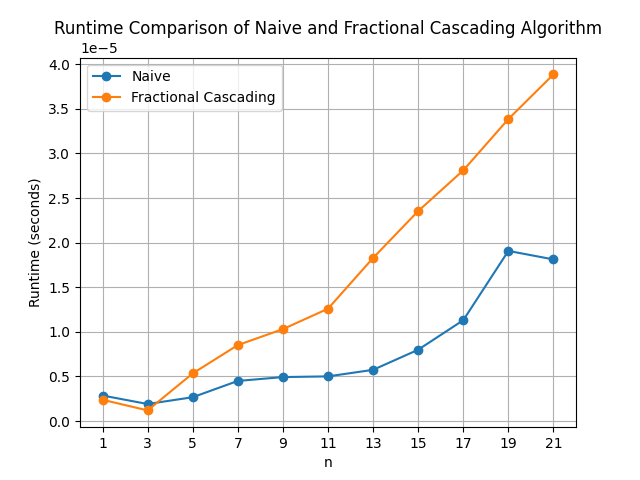
\includegraphics[width=0.7\linewidth]{images/3_1} 

}

\caption{Running time of path 1 on $d=3$.}\label{fig:graph1}
\end{figure}

~

\begin{figure}

{\centering 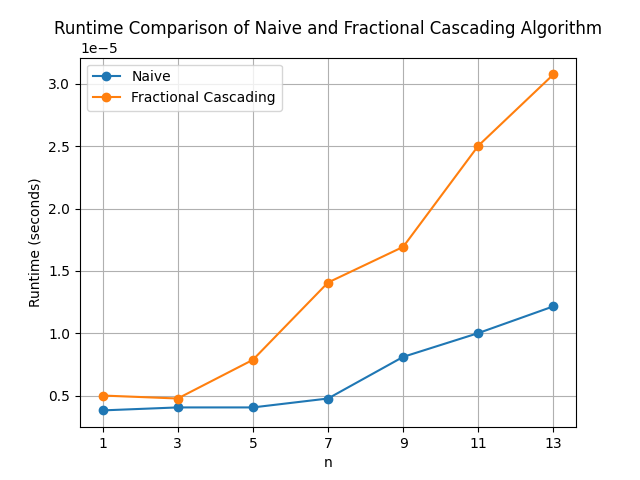
\includegraphics[width=0.7\linewidth]{images/4_1} 

}

\caption{Running time of path 1 on $d=4$.}\label{fig:graph2}
\end{figure}

\begin{figure}

{\centering 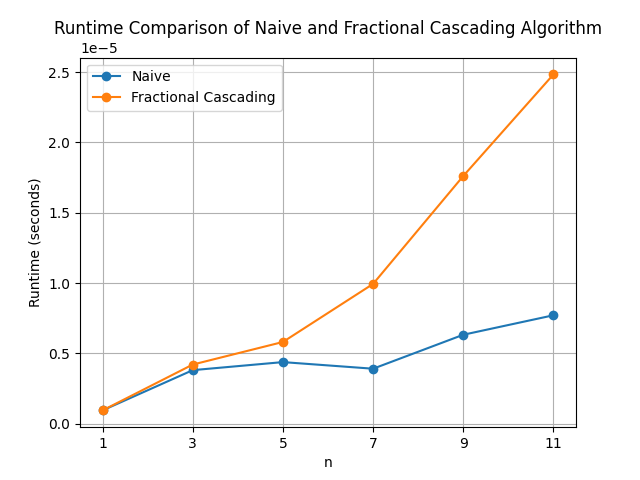
\includegraphics[width=0.7\linewidth]{images/5_1} 

}

\caption{Running time of path 1 on $d=5$.}\label{fig:graph3}
\end{figure}

\begin{figure}

{\centering 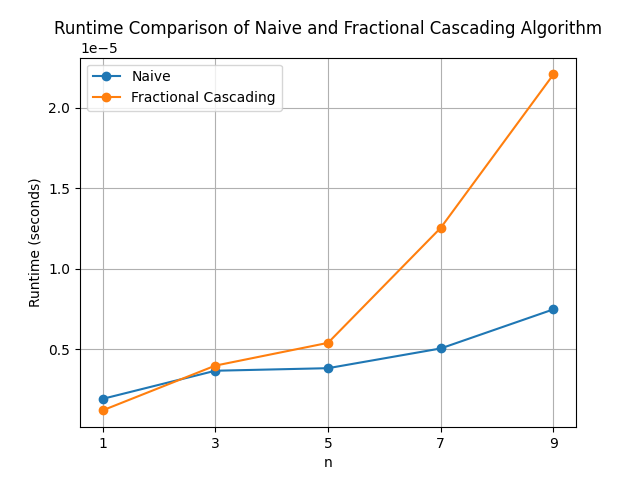
\includegraphics[width=0.7\linewidth]{images/6_1} 

}

\caption{Running time of path 1 on $d=6$.}\label{fig:graph4}
\end{figure}

\hrule

\begin{figure}

{\centering 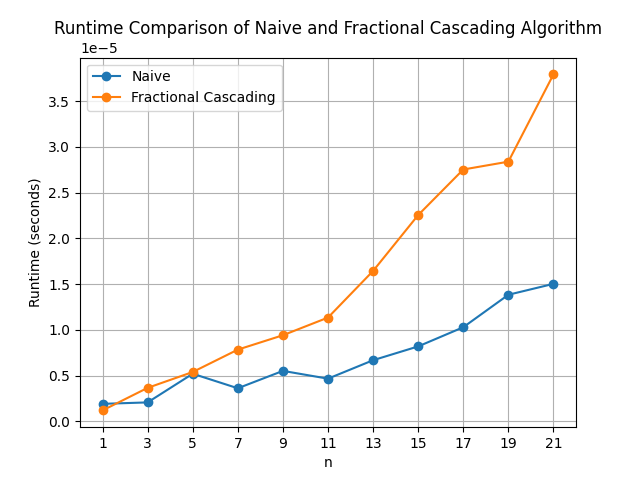
\includegraphics[width=0.7\linewidth]{images/3_2} 

}

\caption{Running time of path 2 on $d=3$.}\label{fig:graph5}
\end{figure}

~

\begin{figure}

{\centering 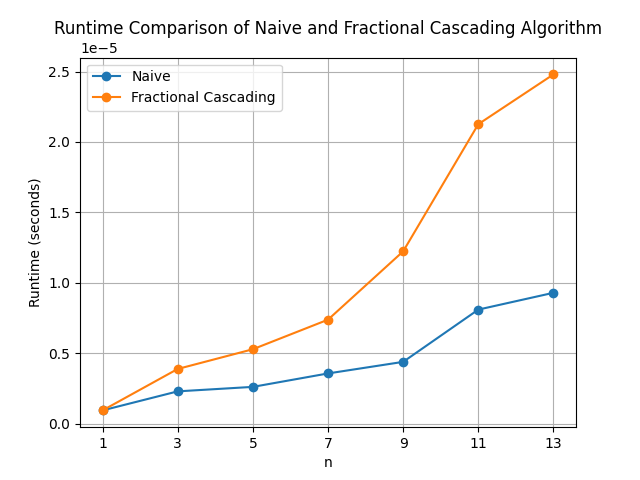
\includegraphics[width=0.7\linewidth]{images/4_2} 

}

\caption{Running time of path 2 on $d=4$.}\label{fig:graph6}
\end{figure}

\begin{figure}

{\centering 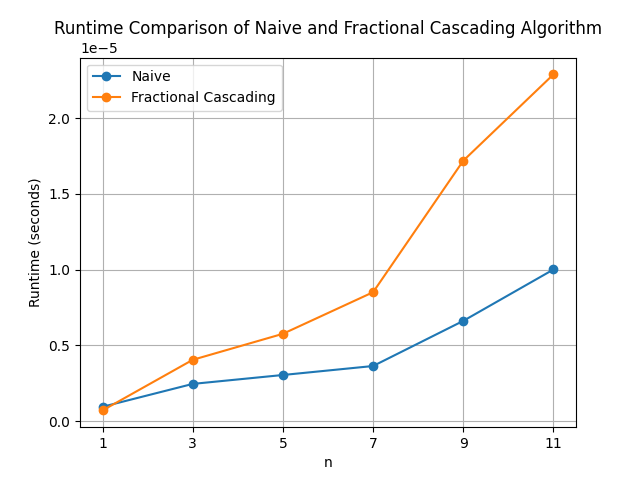
\includegraphics[width=0.7\linewidth]{images/5_2} 

}

\caption{Running time of path 2 on $d=5$.}\label{fig:graph7}
\end{figure}

\begin{figure}

{\centering 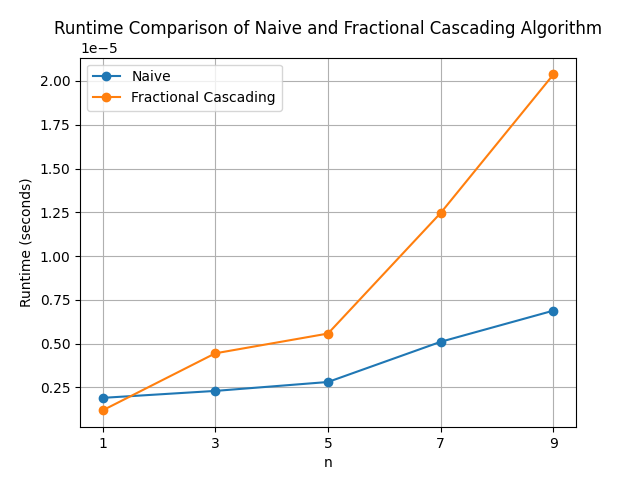
\includegraphics[width=0.7\linewidth]{images/6_2} 

}

\caption{Running time of path 2 on $d=6$.}\label{fig:graph8}
\end{figure}

When $n=1$, the tree is a single vertex $v$ with $C(v)=A(v)$. It is expected that the runtime
of both algorithms should be the same because we do binary search on the same list. However,
the actual running times slightly vary between the two algorithms, and this could be due to
the computing power at the time of measurement.

We observe that the graphs of fractional cascading always have higher slope than the graph of
naive algorithm. As $n$ gets large, the running time of fractional cascading increases much
faster than the running time of naive algorithm. This is not what we expected because in a
path, which is a subgraph $(V', E')$ of the N-ary tree $(V,E)$, naive algorithm runs in
$O(|V'|\log_{} n)$ time while fractional cascading has running time of $O(|V'|+\log_{} n)$.
Given limited computing power, the maximum number of nodes that I can get to is just over 2
million nodes, which is equivalent to $n=21$ when $d=3$.

The question is as $n$ gets larger, will there ever be the point that fractional cascading
outperforms the naive algorithm. Based on the graphs that we acquired, it is unlikely that
growth rate of fractional cascading running time seems so much higher than that of the naive 
algorithm.

\hypertarget{section4}{%
\section{\texorpdfstring{4 \enspace Conclusion}{4 Conclusion}}\label{section4}}

The algorithm did not work as expected.

\end{document}
